\documentclass[UTF8,11pt,twocolumn]{ctexart}

\usepackage[a4paper,margin=0.68in,columnsep=0.28in]{geometry}
\usepackage{amsmath,amssymb}
\usepackage{booktabs}
\usepackage{array}
\usepackage{tabularx}
\usepackage{enumitem}
\usepackage{graphicx}
\usepackage{cuted}
\usepackage{titling}
\usepackage{titlesec}
\usepackage{tikz}
\usetikzlibrary{arrows.meta,positioning,fit,shapes.geometric,calc}
\usepackage[hidelinks]{hyperref}
\graphicspath{{figures/}}

\setlength{\parindent}{1.5em}
\setlength{\parskip}{0pt}
\linespread{0.98}
\setlength{\textfloatsep}{8pt plus 2pt minus 2pt}
\setlength{\dbltextfloatsep}{8pt plus 2pt minus 2pt}
\setlength{\abovecaptionskip}{4pt}
\setlength{\belowcaptionskip}{0pt}
\setlist[itemize]{topsep=2pt,itemsep=2pt,parsep=0pt,partopsep=0pt,leftmargin=1.4em}
\setlist[enumerate]{topsep=2pt,itemsep=2pt,parsep=0pt,partopsep=0pt,leftmargin=1.4em}
\setlength{\droptitle}{-1.8em}

\ctexset{
  section = {
    format = \Large\bfseries,
    beforeskip = 1.0ex plus .2ex minus .1ex,
    afterskip = 0.6ex plus .1ex,
  },
  subsection = {
    format = \large\bfseries,
    beforeskip = 0.8ex plus .2ex minus .1ex,
    afterskip = 0.4ex plus .1ex,
  },
}
\titlespacing*{\paragraph}{0pt}{0.4ex}{0.3ex}
\titlespacing*{\subparagraph}{0pt}{0.4ex}{0.3ex}

\title{TRACE-RAG：面向复杂问答的自适应图文融合检索增强生成框架}
\author{待补充}
\date{}

\begin{document}
\maketitle

\begin{abstract}
检索增强生成（RAG）已经成为缓解大语言模型幻觉的重要方法，但在复杂问答场景中仍存在检索策略固定、缺少答案验证和输出格式不稳等问题。本文提出 TRACE-RAG，一个统一的图文融合 agentic RAG 框架，将查询理解、自适应路由、证据融合、多智能体重生成、Critic 反馈和答案规范化整合为闭环流程。我们在 PopQA 和 MuSiQue 上验证了该方法，结果表明 TRACE-RAG 在 MuSiQue 上具有稳定优势，并且在 paired-retriever 与消融分析中显示出清晰的模块贡献。
\end{abstract}

\noindent\textbf{关键词：} 检索增强生成；复杂问答；图文融合；迭代检索；答案规范化

\begin{figure*}[t]
\centering
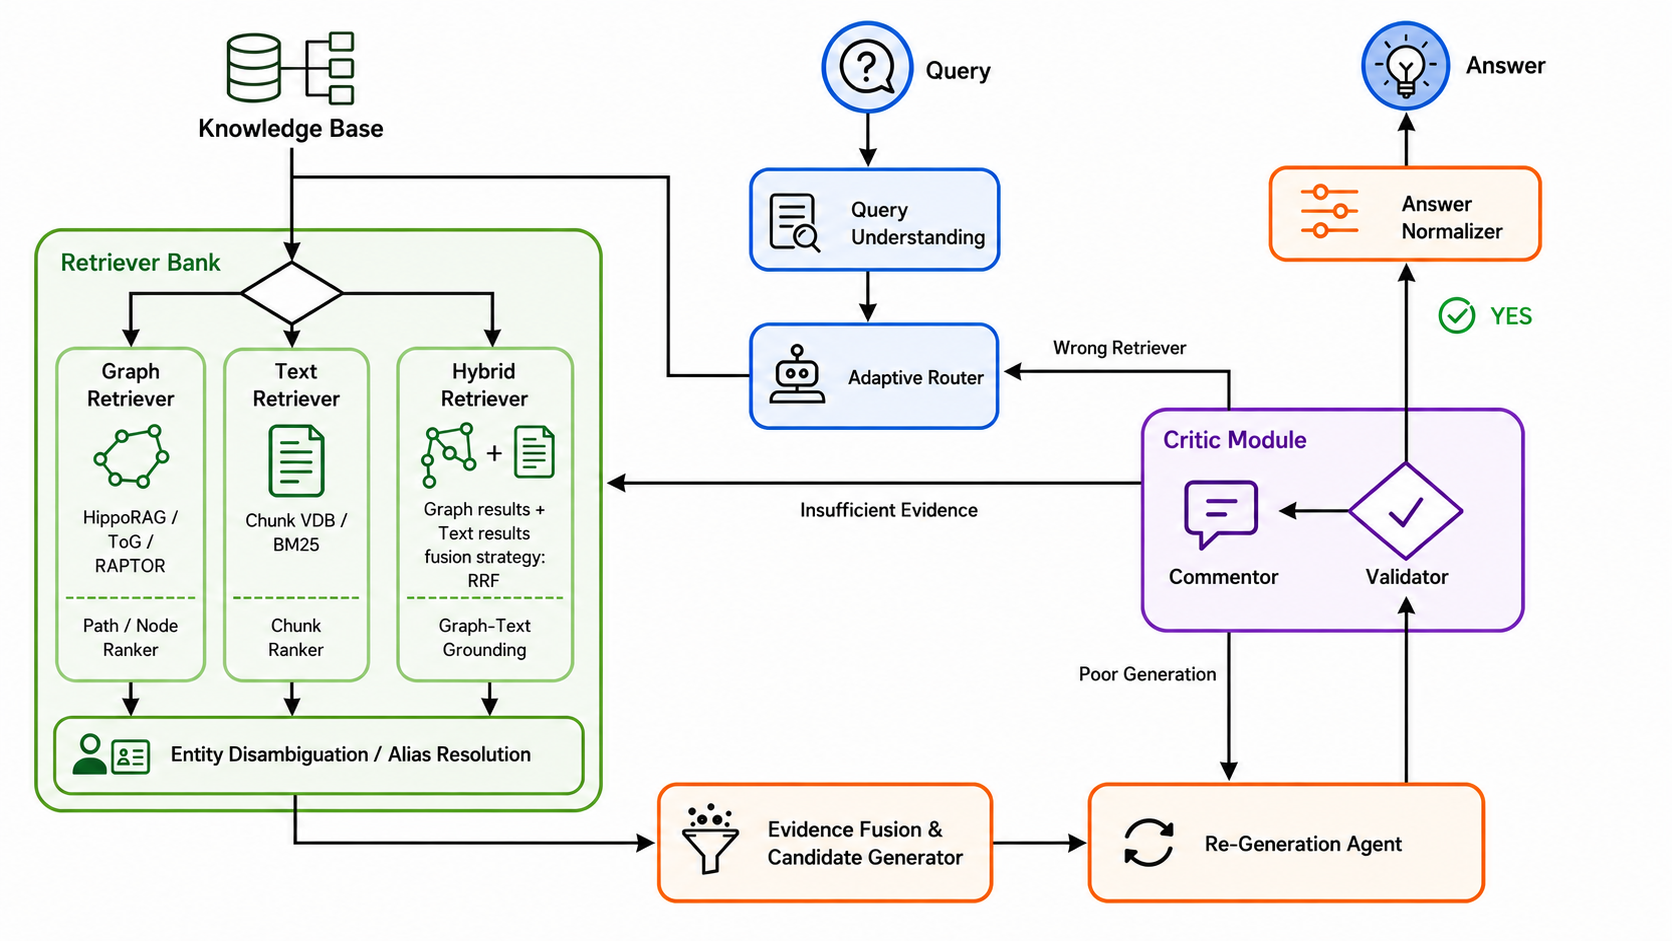
\includegraphics[width=\textwidth]{b41a55c0-335e-4613-8492-ff1dd073d82b.png}
\caption{TRACE-RAG 的整体架构。系统围绕检索选择、证据融合、答案重生成、Critic 验证与答案规范化形成闭环。}
\label{fig:architecture}
\end{figure*}

\section{引言}

\subsection{研究动机}

传统 RAG \cite{rag2020,robertson2009probabilistic,karpukhin2020dpr} 主要通过检索外部知识缓解幻觉，但面对复杂问答时，固定检索路径往往无法适应不同问题类型。实体属性类问题、多跳推理问题以及需要跨文档证据组合的问题，对证据形态的要求并不相同；如果系统始终使用同一种检索策略，就很难在所有任务上都保持稳定表现。

\subsection{研究背景与现状}

图检索与图增强 RAG \cite{jimenez2024hipporag,hu2024grag,shen2024gear,yao2023tot,sarthi2024raptor} 说明结构化证据对于多跳推理的重要性，但图构建质量、覆盖率和长尾实体稀疏性仍限制了其稳定性。与此同时，自我反思与主动检索工作 \cite{asai2023selfrag,jiang2023flare} 进一步表明，系统应当具备“证据不足则继续检索”的能力，而不是把一次检索结果直接视为最终答案。换言之，复杂问答更需要闭环控制，而不是单次生成。

\subsection{研究问题}

围绕现有方法的局限，本文关注三个研究问题：第一，能否在图检索、文本检索与混合检索之间根据问题特征动态切换；第二，能否把证据充分性、生成质量与检索错误显式分离，从而构建可迭代修正的闭环；第三，能否通过答案规范化降低评测时的格式波动，提升指标稳定性。

\subsection{主要贡献}

基于 DIGIMON 的统一图文 RAG 基础，本文提出 TRACE-RAG，并围绕自适应路由、多智能体式重生成、Critic 驱动迭代和答案规范化形成完整闭环。本文的主要贡献如下：

\begingroup
\raggedright
\begin{itemize}[leftmargin=1.5em]
  \item 提出 TRACE-RAG，一个面向复杂问答的统一图文 agentic RAG 框架。
  \item 设计 ReGenerationAgent、Critic、Commendor 和 AnswerNormalizer 的协同流程，其中 ReGenerationAgent 仅在 poor generation 情况下触发。
  \item 在 PopQA 与 MuSiQue 上进行系统评测，并提供 paired-retriever 和 leave-one-out 消融分析。
\end{itemize}
\endgroup

图1给出了 TRACE-RAG 的主架构。图中左侧的 Retriever Bank 负责召回图证据、文本证据与混合证据；中间的 Query Understanding 与 Adaptive Router 负责判定该使用何种检索路径；下方的 Evidence Fusion 与 Re-Generation Agent 负责将证据整合并生成候选答案；右侧的 Critic Module、Commendor 与 AnswerNormalizer 则负责显式验证、失败归因和输出规范化。该图强调的不是模块数量，而是闭环控制逻辑：TRACE-RAG 试图把复杂问答分解为可诊断、可修复、可比较的多个环节。

\subsection{文章结构}

本文余下部分组织如下：第 2 节回顾相关工作；第 3 节介绍 TRACE-RAG 的方法设计；第 4 节给出实验设置；第 5 节报告主要结果与消融分析；第 6 节展示典型案例；第 7 节讨论局限性；第 8 节总结全文。

\section{相关工作}

\subsection{检索增强生成}
检索增强生成通常采用“检索 - 拼接 - 生成”的三段式范式：首先从外部语料中召回候选证据，再将证据拼接到提示词中，最后由生成模型给出答案。BM25、DPR 及其变体构成了该方向最常见的两类基础检索器，前者强调词项匹配，后者强调语义相似。该类方法结构简单、实现成本低，适合作为大多数开放域问答任务的起点。然而，当问题需要跨句、跨段或跨文档组合证据时，单一文本检索容易受到召回粒度、冗余上下文和证据覆盖率的限制，进而影响生成结果的稳定性。换言之，传统 RAG 的核心问题并不只是“检索是否存在”，而是“检索到的证据是否足以支持复杂推理”。

\subsection{图检索增强生成}
图检索增强生成试图将实体、关系和路径结构显式编码到知识图或推理图中，以支持多跳推理与结构化证据定位。HippoRAG、GRAG、GeAR、ToG、RAPTOR 等工作表明，在实体关系明确、路径依赖较强的场景中，图结构通常比纯文本更有优势，因为它能保留“谁与谁相关”“事件如何连接”这类显式约束。Zhou 等人还从统一框架视角系统比较了图检索 RAG 方法，强调了不同图方法在统一设置下的行为差异 \cite{zhou2025graphragunified}。不过，图方法也面临一系列现实瓶颈：其一，图构建质量高度依赖抽取与对齐过程；其二，长尾实体与冷门关系往往稀疏；其三，图检索对噪声边、错误边和别名问题较为敏感。因此，图检索更适合作为复杂问答中的结构化支撑，而不一定能单独覆盖所有任务。

\subsection{Agentic 与迭代式 RAG}
Agentic 与迭代式 RAG 进一步将“是否继续检索”显式纳入推理过程。Self-RAG、FLARE 以及 AGENT-G 等方法表明，模型不仅可以回答问题，还可以在回答过程中对证据充分性、自身置信度和答案可靠性进行判断，并在需要时主动发起下一轮检索或修正 \cite{asai2023selfrag,jiang2023flare,agentg2025}。这类方法的共同点在于，它们不把第一次检索结果视为终局，而是将检索视为可重复、可调整的过程。相比之下，若系统缺少这类闭环控制，就容易在证据不足时过早输出答案，从而产生高置信度误答。TRACE-RAG 继承了这一方向的核心思想，并将其与图文融合和失败归因进一步结合。

\subsection{小结}

综合来看，文本 RAG 解决的是“如何找证据”的基础问题，图 RAG 解决的是“如何利用结构化关系”的问题，而 agentic RAG 解决的是“何时补检索、如何修正”的问题。现有工作已经分别在这些方向上取得进展，但仍缺少一个同时覆盖检索路由、图文融合、重生成、验证和输出规范化的统一闭环。本文提出的 TRACE-RAG 正是针对这一空白展开设计的。

\section{方法}

\subsection{总体架构}

TRACE-RAG 的整体流程可以概括为：

\[
\begin{aligned}
q &\rightarrow \text{QueryUnderstanding} \rightarrow \text{Retriever Bank} \rightarrow \\
  &\rightarrow \text{Evidence Fusion} \rightarrow \text{ReGenerationAgent} \rightarrow \\
  &\rightarrow \text{Critic} \rightarrow \text{AnswerNormalizer} \rightarrow a^*
\end{aligned}
\]

其中，$q$ 是输入问题，$a^*$ 是最终输出答案。若 Critic 判断当前答案仍不可靠，则系统会在最多 $R$ 轮内继续触发补检索与再生成。当前实现中，$R$ 默认为 3。

为便于形式化描述，记第 $t$ 轮检索得到的证据为 $E_t$，重生成输出为 $\hat{a}_t$，Critic 评分为 $s_t$，答案规范化函数为 $\mathcal{N}(\cdot)$，则 TRACE-RAG 的一轮闭环更新可写为：

\[
\begin{aligned}
E_t &= \mathcal{R}(q, t), \\
\hat{a}_t &= \mathcal{G}(q, E_t), \\
s_t &= \mathcal{C}(q, E_t, \hat{a}_t), \\
a_t &= \mathcal{N}(\hat{a}_t), \\
a^* &= a_t \quad \text{if } s_t \ge \tau \text{ or } t = R .
\end{aligned}
\]

其中，$\mathcal{R}$ 表示检索模块，$\mathcal{G}$ 表示重生成模块，$\mathcal{C}$ 表示 Critic，$\tau$ 为停止阈值。

如图1所示，TRACE-RAG 不是简单串联多个模块，而是把系统拆成三层：第一层是路由层，由 Query Understanding 与 Adaptive Router 负责判断问题类型和检索偏好；第二层是证据层，由 Retriever Bank、Entity Disambiguation / Alias Resolution 与 Evidence Fusion 负责把异构召回结果整理成统一上下文；第三层是反馈层，由 Re-Generation Agent、Critic、Commendor 与 AnswerNormalizer 负责答案生成、失败归因与输出规范化。

这样的设计有两个直接好处。第一，它把“错误发生在哪里”显式化，便于分析系统瓶颈是来自路由、召回、重生成还是规范化；第二，它让不同模块的职责边界清晰，便于做 leave-one-out 消融并比较其边际贡献。

\subsection{查询理解与自适应路由}

不同问题对证据形态的需求并不相同。实体属性类问题通常更适合图检索，因为答案往往与实体关系直接相关；多跳、背景依赖强的问题则更需要文本检索补充上下文。如果系统对所有问题都采用同一条检索路径，就会在某一类问题上稳定吃亏。

TRACE-RAG 的 QueryUnderstanding 模块对输入问题进行一次 LLM 推断，输出问题的粗粒度结构信息，例如问题域、关键实体、关系线索、时间线索以及检索偏好。Adaptive Router 再根据这些结构信息，在 graph、text、hybrid 三类模式之间选择后续检索分支。这里的“自适应”不是无限制自由路由，而是在当前图方法与文本方法配置下，动态决定更偏向哪一类证据。

从实现角度看，路由器输出的不是最终答案，而是后续检索策略。它回答的是“先从哪里找”，而不是“答案是什么”。这样做的好处是把路由错误与生成错误分离开来，便于后续分析和调试。

\subsection{检索器集合与证据融合}

TRACE-RAG 的 Retriever Bank 兼容三类图方法与两类文本方法：

\begin{itemize}[leftmargin=1.5em]
  \item 图检索：HippoRAG 风格的实体关系检索、ToG 风格的图遍历检索、RAPTOR 风格的层级摘要检索；
  \item 文本检索：BM25 与 VDB；
  \item 混合检索：通过融合策略合并图证据与文本证据。
\end{itemize}

BM25 偏重词项匹配，适合关键词明确的事实问答；VDB 偏重语义相似，适合表达方式变化较大但语义关联明显的问题。混合模式下，TRACE-RAG 通过融合图与文两路召回结果，尽量在结构约束与语义补充之间取得平衡。

证据融合模块会将检索到的候选片段整理为统一上下文，并构造面向生成模块的输入。其目标不是简单拼接文本，而是尽可能保留支持答案判断的关键信息，减少噪声证据对生成的干扰。结合图1可以更直观地理解这一点：Graph Retriever 输出结构化关系路径，Text Retriever 输出段落级证据，Hybrid Retriever 则通过 RRF 等策略把两类信号合并。随后 Entity Disambiguation / Alias Resolution 把同名实体、别名实体和歧义实体统一到同一语义空间，避免后续生成阶段围绕错误实体展开。

\subsection{ReGenerationAgent}

单次生成在证据不足或证据冲突时容易输出不稳定答案。为降低这一风险，TRACE-RAG 将答案生成拆解为 judge-vote-infer 三个阶段；其中 ReGenerationAgent 只在 Critic 判定为 poor generation 时触发，用来修正证据已经足够但答案表达不稳定的情况：

\begin{itemize}[leftmargin=1.5em]
  \item Judge 阶段：多个 judge 独立阅读证据并给出候选答案与置信度；
  \item Vote 阶段：vote 模块综合多个 judge 的结果，选出更一致的候选；
  \item Infer 阶段：最终 inference agent 基于证据与投票结果输出简洁答案。
\end{itemize}

这一设计的核心目的不是让模型“思考更久”，而是通过并行协作降低单次生成的偶然误差。当前实现默认使用较小规模的 judge/voter 组合，以控制推理成本，因此 ReGenerationAgent 的作用更偏向稳定化，而不是无成本地提升模型能力。

\subsection{Critic 驱动的迭代检索}

Critic 是 TRACE-RAG 闭环的核心。它读取当前候选答案与证据集，对答案是否被证据充分支持进行结构化判断，输出三类决策之一：

\begin{itemize}[leftmargin=1.5em]
  \item \texttt{pass}：当前答案可接受，直接结束；
  \item \texttt{revise}：答案可以小幅修正，但不必重新检索；
  \item \texttt{retrieve\_more}：证据不足，需要继续补检索。
\end{itemize}

与此同时，Commendor 会把失败原因进一步归类为四种标签：
\begin{itemize}[leftmargin=1.5em]
  \item \texttt{insufficient\_evidence}：召回证据不够；
  \item \texttt{wrong\_retriever}：路由或检索器选型不对；
  \item \texttt{poor\_generation}：证据足够但表达质量仍不足；
  \item \texttt{pass}：当前结果可接受。
\end{itemize}
这样做的价值在于把“为什么失败”拆得更细，并为后续消融与案例分析提供统一标签。

实验中我们观察到，TRACE-RAG 的大多数迭代来自证据不足，而不是纯生成失败。这说明当前系统瓶颈仍主要在检索阶段，而不是单纯的语言表达阶段。换言之，TRACE-RAG 的闭环设计不是为了让模型永远输出更长的解释，而是为了在证据不足时主动补检索，在答案质量不足时主动重生成。

一旦 Critic 判断需要补检索，系统就会依据反馈调整检索问题、重选检索分支，并重新进入证据融合与生成流程，直到达到最大轮数或者获得可接受答案。

\subsection{答案规范化}

评测任务通常要求短、直接、可字符串匹配的答案，而生成模型天然倾向于输出解释性文本。若不加规范化，很多实际上答对的样本会因为格式差异而被 EM 判错。为此，TRACE-RAG 在最终输出前引入 AnswerNormalizer，对候选答案做抽取、压缩与格式统一，使结果更接近评测标准。

AnswerNormalizer 的目标不是越短越好，而是保留语义核心并去掉无关解释。它是一个对评测友好的后处理模块，不应被误解为简单的字符串截断。更准确地说，它承担的是“评测接口层”的作用，直接影响 EM、Precision 和字符串一致性。

\section{实验设置}

\subsection{数据集}

为了验证方法在不同复杂度任务上的有效性，本文选择两个公开基准作为实验对象，并覆盖从单事实问答到多跳推理的不同难度区间：

\begin{itemize}[leftmargin=1.5em]
  \item PopQA：以实体属性和事实问答为主，适合测试图检索与事实提取能力；
  \item MuSiQue：以多跳推理为主，适合测试复杂问答、证据组合与迭代修正能力。
\end{itemize}

每个数据集均抽取 200 条样本进行统一评测，便于跨方法、跨模型比较。这个规模约占 PopQA 全集 1399 条的 14.3\%，占 MuSiQue 全集 3000 条的 6.7\%。为保证对比公平，所有方法都在相同样本集上进行评测，并采用统一的答案标准化规则和指标计算方式。整体上，PopQA 更适合观察系统在简单事实问答上的边界，而 MuSiQue 更适合体现 TRACE-RAG 的闭环优势。

\subsection{对比方法}

为了从不同技术路线评估 TRACE-RAG 的实际效果，我们将对比方法划分为三类：

\begin{itemize}[leftmargin=1.5em]
  \item BM25
  \item VDB
  \item HippoRAG
  \item RAPTOR
  \item ToG
  \item AgentG
  \item TRACE-RAG 的多种 graph/text 组合版本
\end{itemize}

这些方法覆盖纯文本检索、图结构检索以及图文混合检索三个层次。TRACE-RAG 并不是与所有方法在完全相同实现细节下比较，而是在可复现配置上尽量统一检索策略、重生成策略和反馈策略，从而更贴近真实系统对比。换言之，我们关心的不是某一个单点检索器的极限分数，而是一个完整闭环系统在复杂问答中的综合表现。

\subsection{模型骨干与评测指标}

实验使用三种模型骨干，以观察方法在不同能力边界和输出风格下的稳定性：

\begin{itemize}[leftmargin=1.5em]
  \item deepseek-v3.2
  \item gpt-4o-mini
  \item gemini-2.5-flash-lite
\end{itemize}

评测指标包括：

\begin{itemize}[leftmargin=1.5em]
  \item Accuracy
  \item Exact Match (EM)
  \item Precision
  \item Recall
  \item F1
\end{itemize}

其中，Accuracy 用于给出总体正确率，EM 用于衡量是否与标准答案字符串完全一致，Precision / Recall / F1 则用于更细致地反映答案覆盖与误召回情况。由于生成式答案常常存在格式波动，因此本文尤其重视 AnswerNormalizer 对 EM 与 Precision 的影响。对于本文这样的系统型方法，表~\ref{tab:system-settings} 汇总了核心实验设置，包括共享的模型、检索与控制参数。

\begin{table}[t]
\centering
\small
\begin{tabular}{ll}
\toprule
设置项 & 取值 \\
\midrule
LLM & gemini-2.5-flash-lite \\
Embedding & BAAI/bge-small-en-v1.5 \\
Judge 数 & 3 \\
Voter 数 & 3 \\
最大迭代轮数 & 3 \\
Judge 分数阈值 & 3.0 \\
Critic 输入 & 使用规范化答案 \\
AnswerNormalizer & 启用 \\
Disambiguation & 启用 \\
BM25 top-k & 10 \\
VDB top-k & 10 \\
\bottomrule
\end{tabular}
\caption{TRACE-RAG 的核心实验设置。图检索分支在各骨干方法内部进一步细分为对应的 top-k 与路由参数，表中列出的是跨实验共享的主控参数。}
\label{tab:system-settings}
\end{table}

\subsection{实现细节}

TRACE-RAG 在当前代码中以固定的图方法与文本方法为基础运行，例如：
\begin{itemize}[leftmargin=1.5em]
  \item \texttt{hipporag + bm25}
  \item \texttt{hipporag + vdb}
  \item \texttt{tog + bm25}
  \item \texttt{tog + vdb}
\end{itemize}
对于 ablation，我们构造了 leave-one-out 版本，分别关闭 Router、ReGeneration、Critic、Commendor、AnswerNormalizer 等模块，以观察各组件对最终效果的边际贡献。所有实验统一采用相同的评测样本、相同的答案后处理规则和相同的停止条件，从而保证不同配置之间的差异主要来自方法本身。

\begin{table}[t]
\centering
\small
\begin{tabularx}{\columnwidth}{@{}>{\raggedright\arraybackslash\bfseries}p{1.45cm}>{\raggedright\arraybackslash}X@{}}
\toprule
检索侧 & HippoRAG 采用 \texttt{er\_graph\_colbert} + FAISS，启用实体向量索引和 entity link chunk，使用 PPR（\texttt{top\_k\_entity\_for\_ppr=8}、\texttt{damping=0.1}、\texttt{top\_k=5}）；ToG 采用 \texttt{er\_graph} + 向量库，启用实体与关系向量索引，\texttt{query\_type=tog}、\texttt{width=3}、\texttt{depth=3}、\texttt{top\_k=3}；RAPTOR 采用 \texttt{tree\_graph\_balanced} + FAISS，\texttt{query\_type=basic}、\texttt{top\_k=5}，并使用 \texttt{selection\_mode=top\_k}、\texttt{start\_layer=5}、\texttt{num\_layers=5}、\texttt{threshold=0.1}、\texttt{max\_iter=10}、\texttt{size\_of\_clusters=10}。文本检索分支中，BM25 与 VDB 的 \texttt{top\_k} 均设为 10。 \\
生成侧 & \texttt{n\_judges=3}、\texttt{n\_voters=3}、\texttt{max\_rounds=3}、\texttt{judge\_score\_threshold=3.0}，并启用 Router、ReGeneration、Critic、Commendor、AnswerNormalizer 和 Disambiguation；\texttt{use\_last\_resort\_guess} 关闭。 \\
评测侧 & MuSiQue 使用 validation split，过滤 \texttt{answerable=False} 样本并对 corpus title 去重；两个数据集均按固定的 200 条样本进行评测，并统一采用答案规范化后的打分流程。 \\
\bottomrule
\end{tabularx}
\caption{TRACE-RAG 的实现设置。表中汇总了方法特定配置、生成配置与评测配置。}
\label{tab:implementation-settings}
\end{table}

\section{实验结果}

\subsection{主结果}

总体上，TRACE-RAG 在 MuSiQue 上的优势最为稳定。在三种模型骨干下，最优 TRACE-RAG 配置均优于对应最强基线：DeepSeek 骨干下，TRACE-RAG \texttt{tog+bm25} 的 F1 从 30.06 提升到 31.44；GPT-4o-mini 骨干下，TRACE-RAG \texttt{hippo+bm25} 的 F1 从 24.90 提升到 31.77；Gemini 骨干下，TRACE-RAG \texttt{tog+bm25} 的 F1 从 20.99 提升到 30.26。

表中的增益统一记为 $\Delta M = M_{\text{TRACE-RAG}} - M_{\text{baseline}}$，用于表示 TRACE-RAG 相对对应基线的绝对变化量。

\begin{table}[t]
\centering
\small
\resizebox{\columnwidth}{!}{%
\begin{tabular}{llrrrr}
\toprule
模型 & 最强 TRACE-RAG vs. 基线 & $\Delta$Acc. & $\Delta$EM & $\Delta$F1 & TRACE-RAG F1 \\
\midrule
DeepSeek & TRACE-RAG \texttt{tog+bm25} vs. ToG & +0.50 & +0.50 & +1.38 & 31.44 \\
GPT-4o-mini & TRACE-RAG \texttt{hippo+bm25} vs. HippoRAG & +2.50 & +5.00 & +6.87 & 31.77 \\
Gemini & TRACE-RAG \texttt{tog+bm25} vs. RAPTOR & +10.00 & +7.50 & +9.27 & 30.26 \\
\midrule
平均 & -- & +4.33 & +4.33 & +5.84 & -- \\
\bottomrule
\end{tabular}%
}
\caption{MuSiQue 主结果。每行比较同一骨干下的最强 TRACE-RAG 配置与最强非 TRACE-RAG 基线。}
\label{tab:musique-main-results}
\end{table}

\begin{figure}[t]
\centering
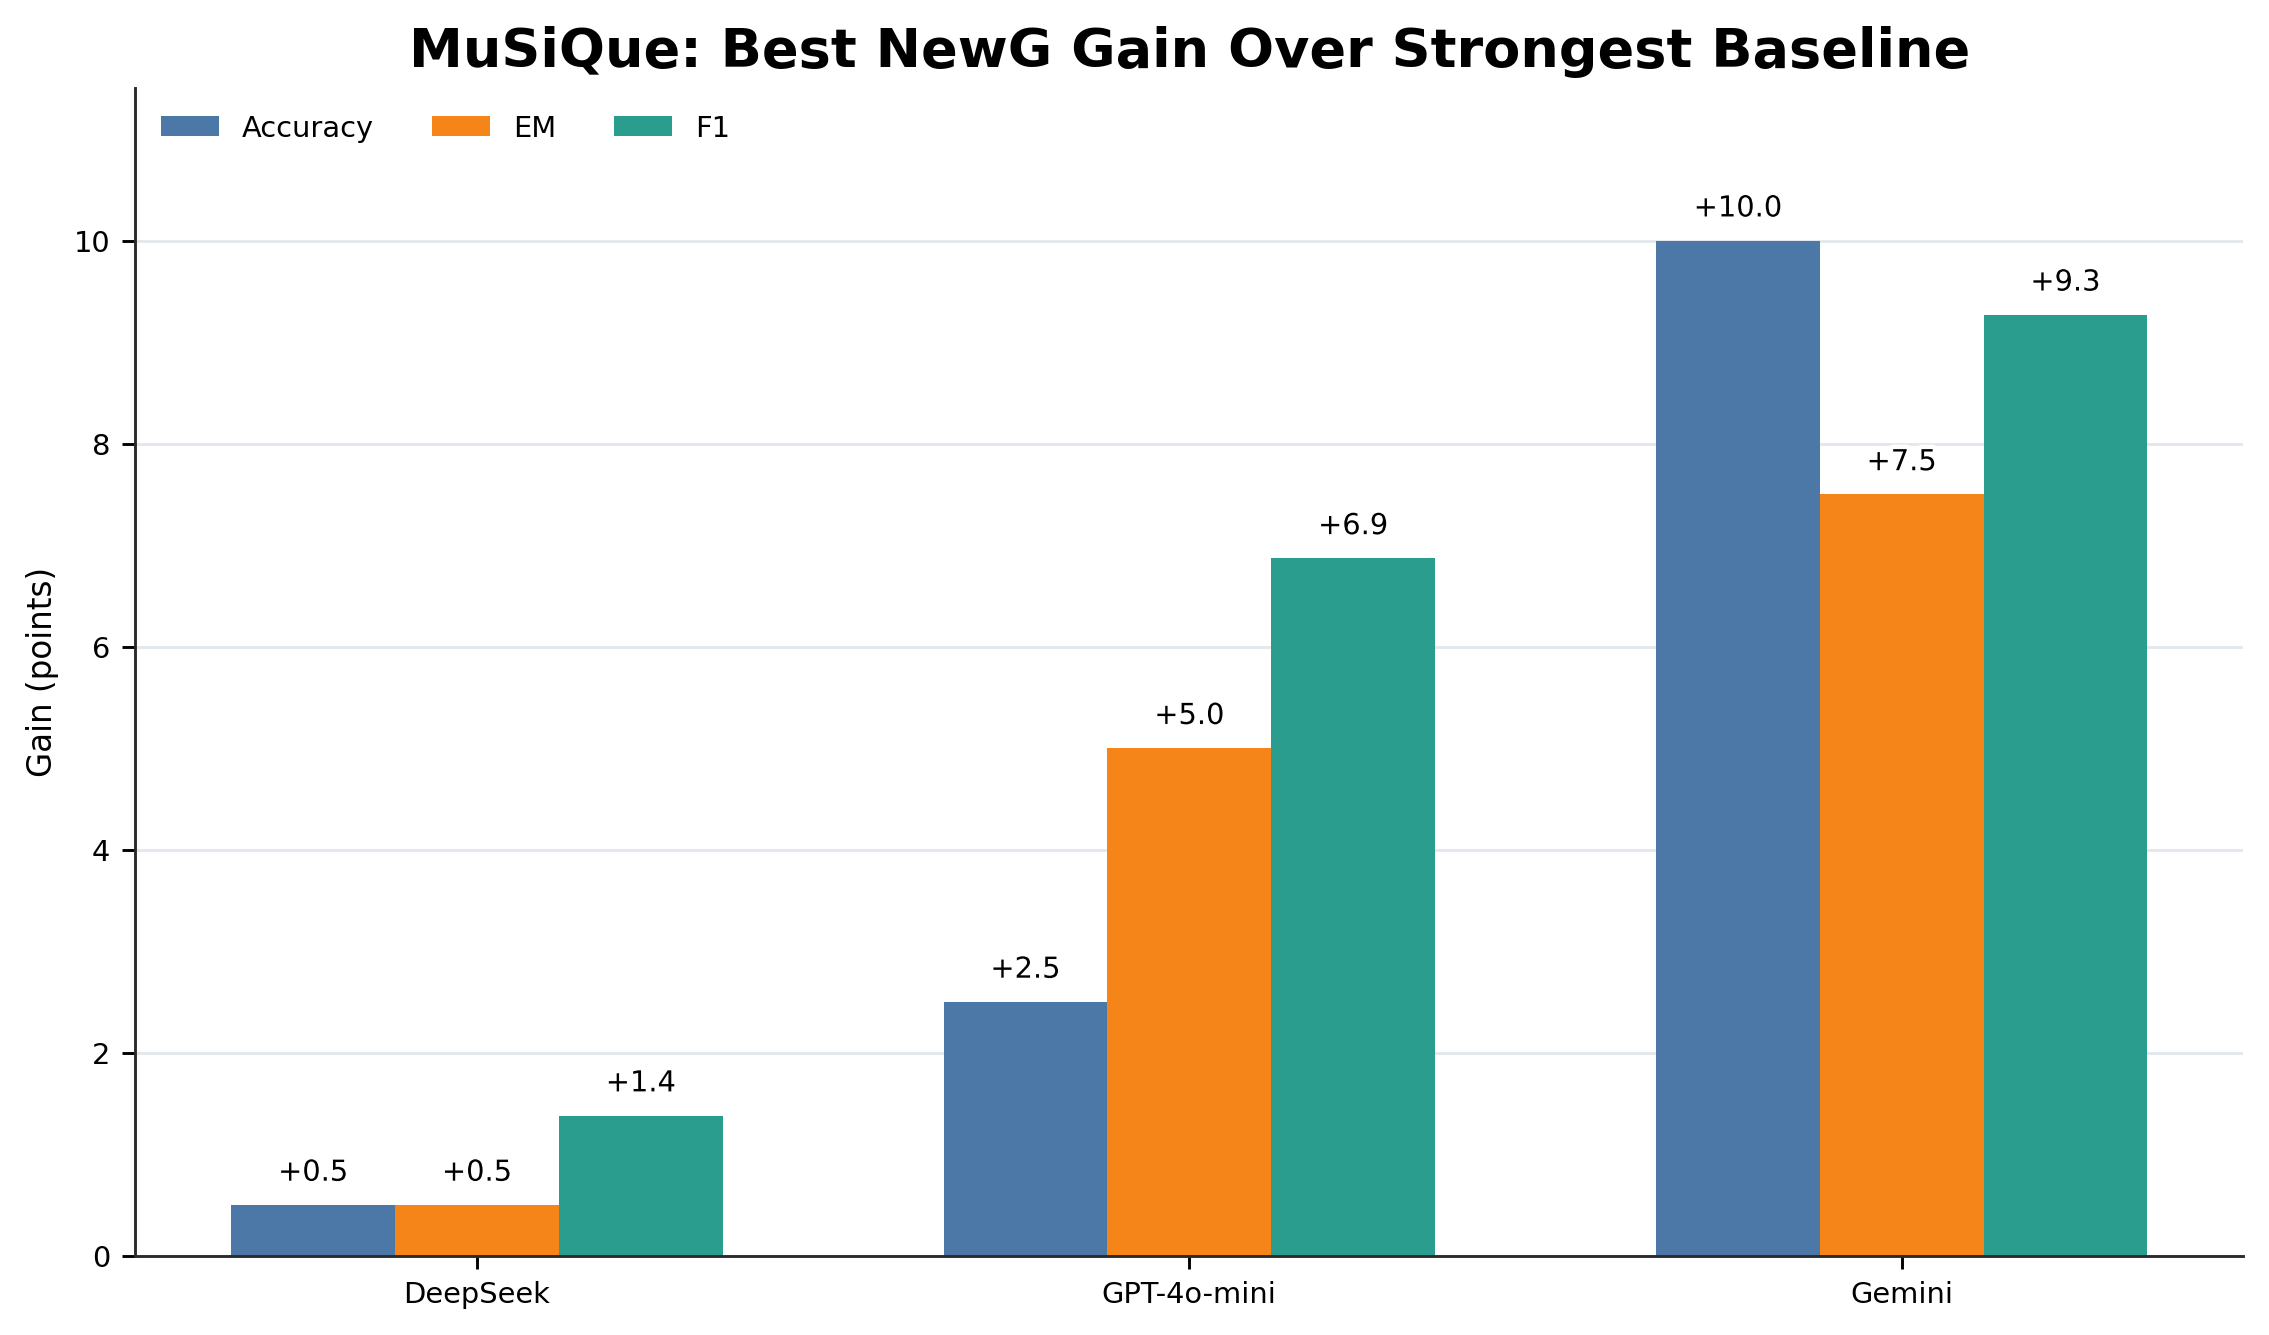
\includegraphics[width=\linewidth]{positive_showcase/panel_musique_best_newg_metric_gains.png}
\caption{MuSiQue 主结果的多指标增益图。该图展示三种骨干下，最强 TRACE-RAG 配置相对最强非 TRACE-RAG 基线在 Accuracy、EM 和 F1 上的变化。}
\label{fig:musique-metric-gains}
\end{figure}

\begin{figure}[t]
\centering
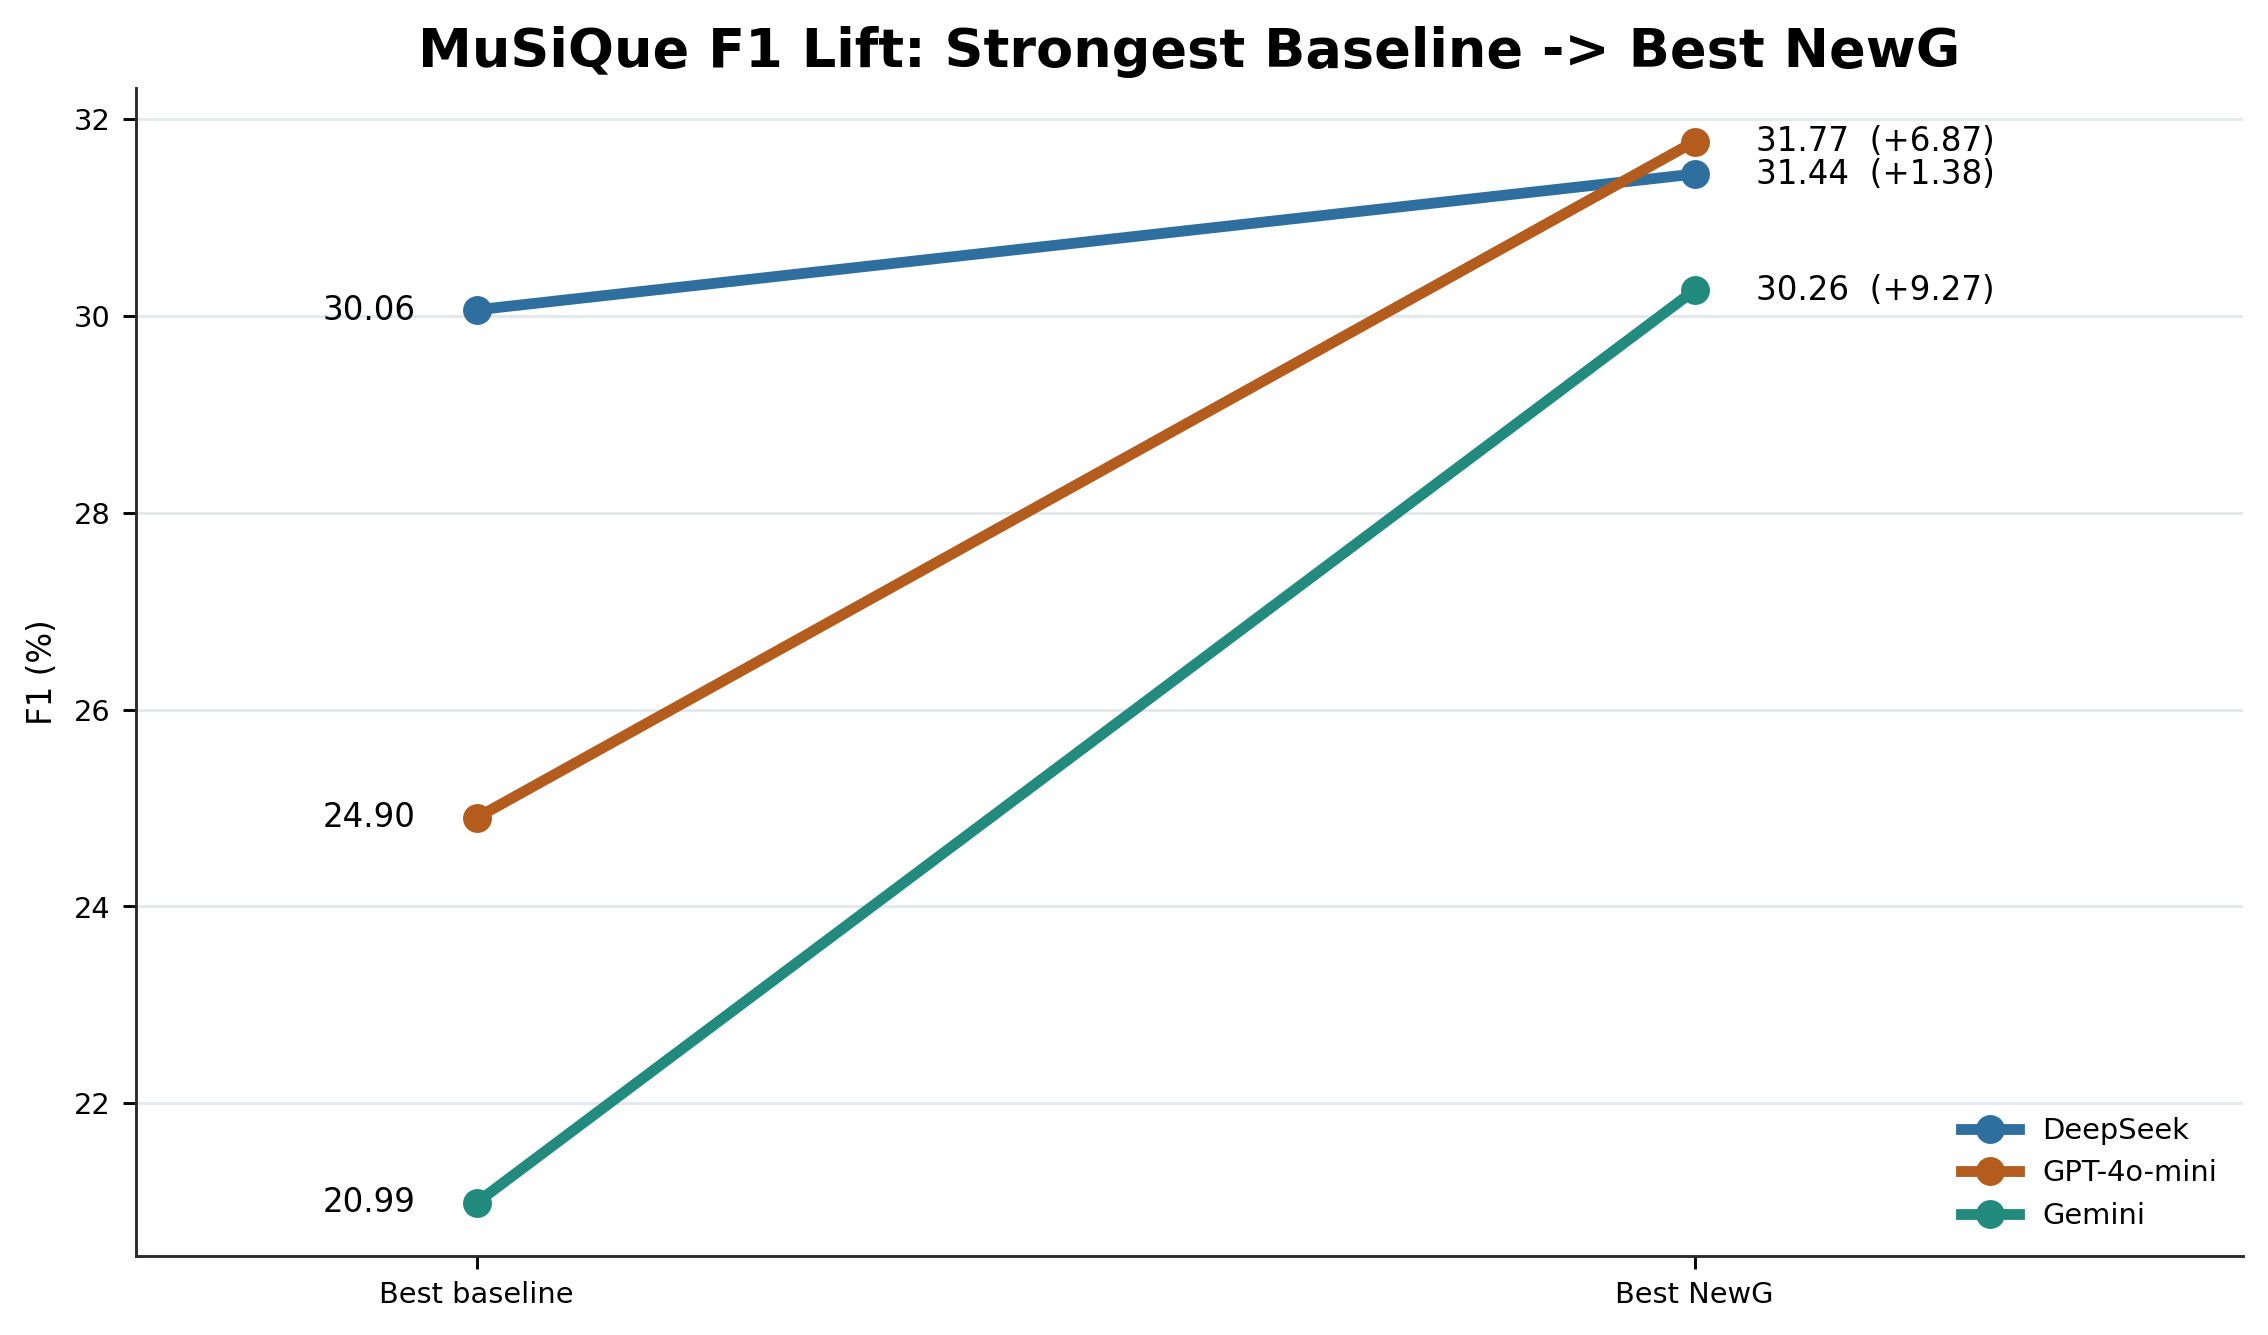
\includegraphics[width=\linewidth]{positive_showcase/panel_musique_best_f1_lift.png}
\caption{MuSiQue 上三种骨干的 F1 提升幅度。该图展示最强 TRACE-RAG 配置相对最强基线的增益。}
\label{fig:musique-f1-lift}
\end{figure}

这组结果说明，TRACE-RAG 的收益并不依赖单一模型骨干，而是能够在不同模型上起到补强作用。特别是在 MuSiQue 这类多跳问答场景中，检索路由、证据融合与迭代修正的组合效应非常明显。换句话说，TRACE-RAG 的价值主要不是把某个单项指标推到极限，而是在复杂任务中提供稳定的系统增益。

PopQA 的结果更为克制。DeepSeek 和 GPT-4o-mini 在最优 TRACE-RAG 配置下分别获得 +0.92 和 +0.20 的 F1 提升，而 Gemini 的最优配置略低于最强基线（-0.35 F1）。这说明 TRACE-RAG 并不是在所有场景下都能大幅超越传统方法；对于更简单、更偏单实体事实的任务，强基线本身已经较强，TRACE-RAG 的主要作用更多体现为稳健性而不是绝对领先。

\begin{table}[t]
\centering
\small
\resizebox{\columnwidth}{!}{%
\begin{tabular}{llrrrr}
\toprule
模型 & 最强 TRACE-RAG vs. 基线 & $\Delta$Acc. & $\Delta$EM & $\Delta$F1 & TRACE-RAG F1 \\
\midrule
DeepSeek & TRACE-RAG \texttt{hippo+bm25} vs. BM25 & +0.00 & -0.50 & +0.92 & 29.78 \\
GPT-4o-mini & TRACE-RAG \texttt{hippo+bm25} vs. BM25 & -1.00 & -0.50 & +0.20 & 29.06 \\
Gemini & TRACE-RAG \texttt{hippo+bm25} vs. HippoRAG & -2.00 & +0.00 & -0.35 & 27.50 \\
\bottomrule
\end{tabular}%
}
\caption{PopQA 稳健性结果。TRACE-RAG 在事实型问答上保持竞争力，但并未对每个骨干都稳定超过最强基线。}
\label{tab:popqa-robustness-results}
\end{table}

因此，论文叙述上应当把 MuSiQue 作为主战场，把 PopQA 定位为边界条件与稳健性测试。这样的表述更符合实际结果，也更能体现方法适用范围。

\subsection{Paired-Retriever 分析}

为了进一步分析 TRACE-RAG 是否真的优于其所依附的图检索基线，我们做了 paired-retriever 分析。结果显示，在 36 组对照中，TRACE-RAG 有 25 组优于对应基线，胜率达到 69.4\%，平均 F1 变化为 +4.78。若只统计正增益样本，平均提升达到 +7.67 F1。

\begin{table}[t]
\centering
\small
\resizebox{\columnwidth}{!}{%
\begin{tabular}{lllrrr}
\toprule
数据集 & 模型 & Pair & Baseline F1 & TRACE-RAG F1 & $\Delta$F1 \\
\midrule
MuSiQue & Gemini & tog+bm25 & 7.71 & 30.26 & +22.55 \\
MuSiQue & Gemini & tog+vdb & 7.71 & 26.94 & +19.23 \\
PopQA & Gemini & tog+bm25 & 11.97 & 25.97 & +14.00 \\
PopQA & Gemini & tog+vdb & 11.97 & 24.71 & +12.74 \\
MuSiQue & DeepSeek & hippo+vdb & 17.28 & 30.01 & +12.73 \\
MuSiQue & DeepSeek & hippo+bm25 & 17.28 & 28.42 & +11.14 \\
\bottomrule
\end{tabular}%
}
\caption{最大的 paired-retriever 增益。每行比较 TRACE-RAG 变体与其图组件所依附的图检索基线。}
\label{tab:paired-retriever-gains}
\end{table}

\begin{figure}[t]
\centering
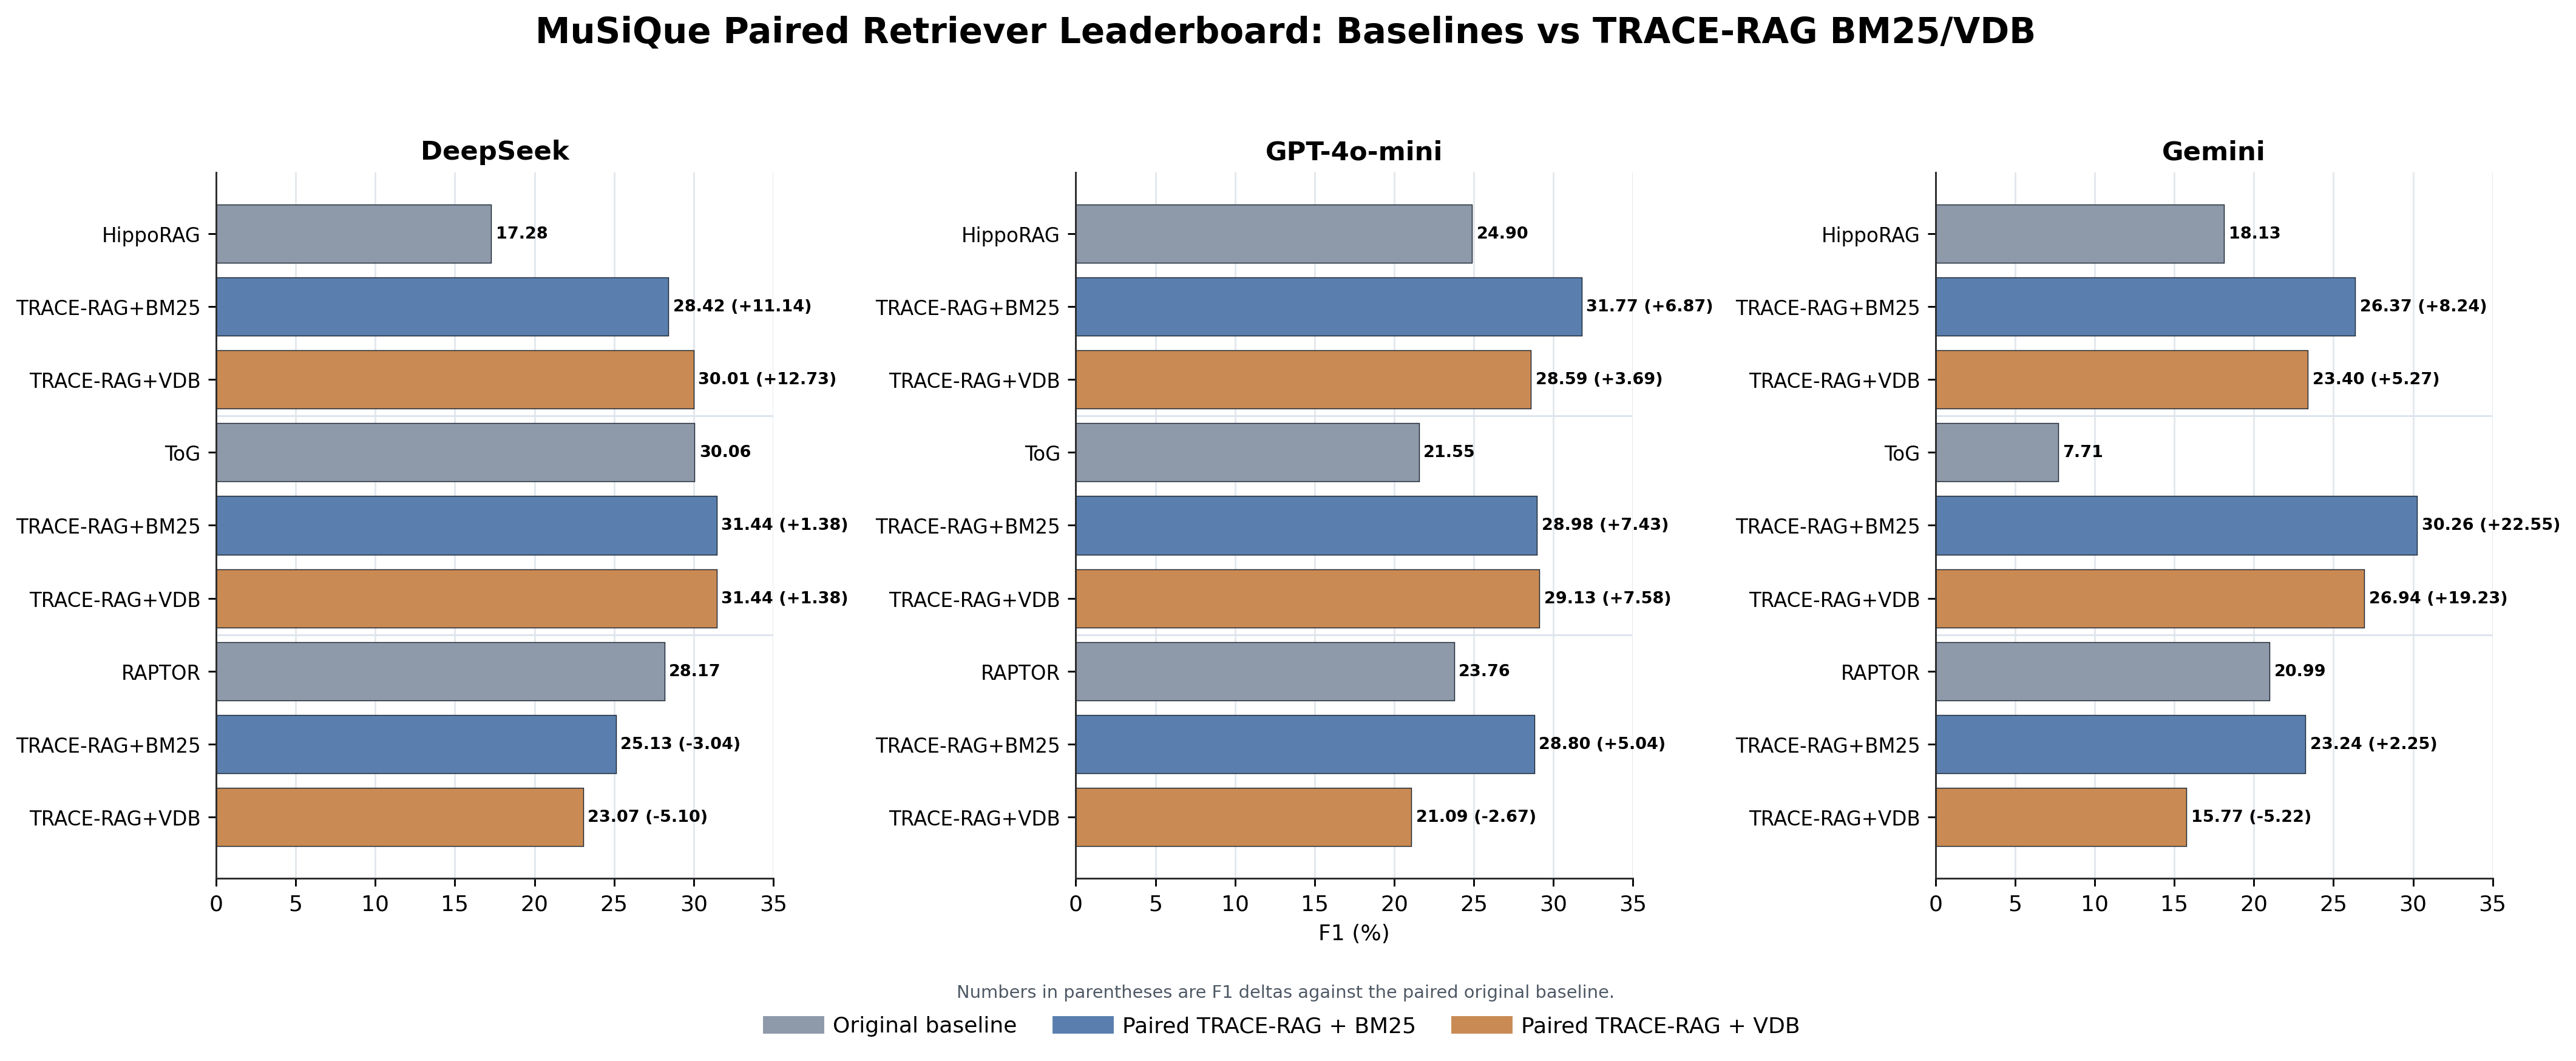
\includegraphics[width=\linewidth]{positive_showcase/showcase_musique_leaderboard.png}
\caption{MuSiQue 的 paired-retriever 排行图。每个基线都与其对应的 TRACE-RAG+BM25 和 TRACE-RAG+VDB 变体进行比较。}
\label{fig:paired-leaderboard}
\end{figure}

这一结果的重要性在于，它表明 TRACE-RAG 的收益并不只是来自“选到了更强的底座”，而是来自图文融合、重生成和反馈闭环共同带来的额外增益。特别是在图基线较弱或不稳定时，TRACE-RAG 往往能够补上缺失证据，从而显著改善最终结果。

\subsection{消融分析}

leave-one-out 消融表明，Critic 与 AnswerNormalizer 是当前最稳定、最可解释的两个关键模块。以 Gemini + \texttt{hippo+bm25} 为例：

\begin{table}[t]
\centering
\small
\resizebox{\columnwidth}{!}{%
\begin{tabular}{llrrrrr}
\toprule
数据集 & 移除模块 & $\Delta$Acc. & $\Delta$EM & $\Delta$Prec. & $\Delta$Rec. & $\Delta$F1 \\
\midrule
MuSiQue & Critic & +4.50 & +4.00 & +5.37 & +5.50 & +5.33 \\
MuSiQue & Answer normalizer & -3.50 & +6.50 & +5.17 & +0.68 & +3.59 \\
PopQA & Critic & +2.50 & +2.00 & +2.25 & +0.83 & +1.04 \\
PopQA & Answer normalizer & -7.00 & +38.50 & +21.46 & -4.19 & +1.45 \\
\bottomrule
\end{tabular}%
}
\caption{关键 leave-one-out 消融效应。数值为 full system 减去 ablated variant，正值表示移除该模块会使对应指标下降。}
\label{tab:key-ablation-effects}
\end{table}

\begin{figure}[t]
\centering
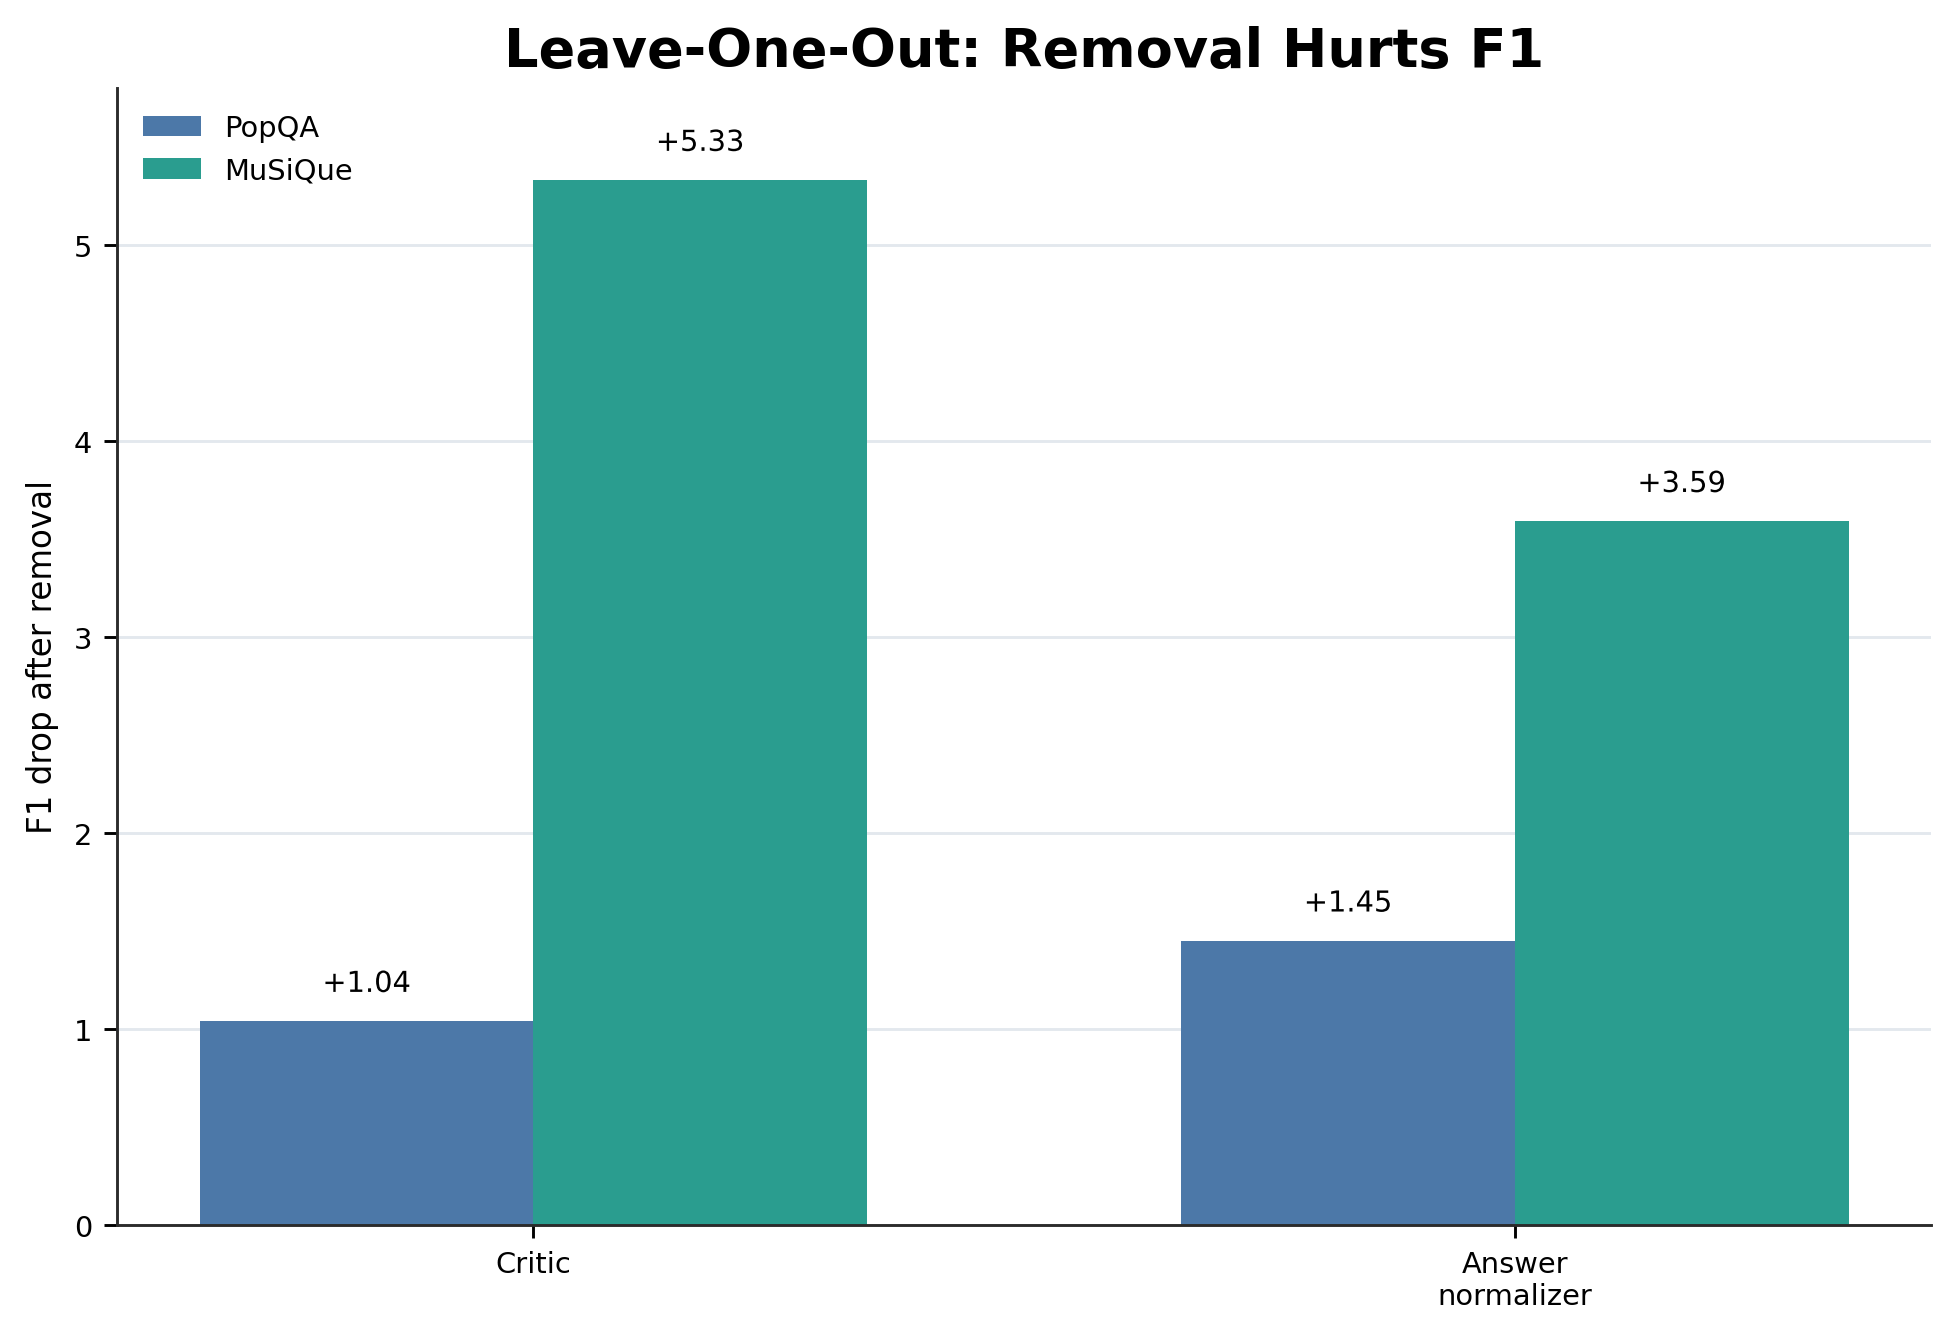
\includegraphics[width=\linewidth]{positive_showcase/panel_leave_one_out_removal_hurts_f1.png}
\caption{Leave-one-out 消融图。移除 Critic 或 AnswerNormalizer 会在 PopQA 和 MuSiQue 上带来最大的 F1 下降。}
\label{fig:loo-ablation}
\end{figure}

\begin{itemize}[leftmargin=1.5em]
  \item 去掉 Critic 后，MuSiQue 的 F1 下降 5.33，PopQA 的 F1 下降 1.04；
  \item 去掉 AnswerNormalizer 后，MuSiQue 的 EM 下降 6.50，PopQA 的 EM 下降 38.50；
  \item AnswerNormalizer 同时对 Precision 也有明显帮助，说明它并非只是格式修饰，而是在统一输出边界、降低字符串噪声。
\end{itemize}

相比之下，Router、ReGenerator、Commendor 的收益更加依赖具体数据集和问题类型。更准确地说，TRACE-RAG 的模块贡献呈现出明显的任务依赖性：Critic 和答案规范化更像通用收益模块，而路由和重生成更像场景敏感模块。

这一结论与图1结构是一致的。图中位于中间的路由与检索链路负责把证据带进来，但真正决定系统能否稳定输出的，往往是右侧反馈链路是否足够敏感、是否能及时识别失败类型。因此，消融结果不是在证明某个模块“无用”，而是在说明 TRACE-RAG 的性能由主检索链路和控制反馈链路共同决定。

\section{案例分析}

为了避免只报告平均分而掩盖系统的真实行为，本节选取服务器上真实运行日志中的两个成功样本和一个失败样本。三者分别对应多轮修正、路由切换和图检索偏置三类典型情形，能够较好地说明 TRACE-RAG 的优势与边界。表~\ref{tab:case-summary} 对三条样本的关键信息进行了概括。

\begin{table*}[t]
\centering
\scriptsize
\setlength{\tabcolsep}{4pt}
\renewcommand{\arraystretch}{1.15}
\begin{tabular}{>{\raggedright\arraybackslash}p{1.4cm} >{\centering\arraybackslash}p{0.8cm} >{\raggedright\arraybackslash}p{5.2cm} >{\raggedright\arraybackslash}p{2.6cm} >{\raggedright\arraybackslash}p{5.7cm}}
\toprule
数据集 & ID & 问题 & 结果 & 关键信号 \\
\midrule
MuSiQue & 121 & What county houses the community of Robinson, in the state where Tom Harkin was from? & Delaware County & 3 轮 graph 推理，前两轮 Critic 连续返回 \texttt{retrieve\_more}，第三轮 \texttt{pass}，说明系统在证据补全后能够稳定收敛。 \\
PopQA & 183 & In what city was Robert Zawada born? & Jedlnia-Letnisko & \texttt{graph} \textrightarrow{} \texttt{hybrid} 路由切换，第一轮 \texttt{revise}，第二轮 \texttt{retrieve\_more}，第三轮 \texttt{pass}，体现出较强的自适应纠正能力。 \\
MuSiQue & 0 & Which network subsidiary broadcasts the weeknight evening news show in part named after the network that aired Crowd Rules? & CNBC / CNBC Asia & 3 轮均偏向 graph 路由，Critic 多次要求补证，但最终答案被压缩为更泛化的上位实体，暴露出粒度不足问题。 \\
\bottomrule
\end{tabular}
\caption{论文中使用的代表性真实服务器案例。前两个是成功修正案例，第三个是典型的近失误失败案例。}
\label{tab:case-summary}
\end{table*}

\paragraph{成功样本一：多轮图检索后完成纠正的地理问答。}
该样本来自 MuSiQue，样本编号为 121，问题为“\emph{What county houses the community of Robinson, in the state where Tom Harkin was from?}”，标准答案为 \emph{Delaware County}。这个问题需要先解析 Tom Harkin 的出生州，再在州内完成社区到县的定位，属于典型的两跳地理问答。实际运行中，TRACE-RAG 连续进行了 3 轮 graph 推理，前两轮已定位到 Iowa 与 \emph{Delaware County, Iowa}，但 Critic 仍返回 \texttt{retrieve\_more}；直到第三轮在补充完整图证据后，系统才最终 \texttt{pass} 并稳定收敛到 \emph{Delaware County}。

\paragraph{成功样本二：路由切换后修正成功的跨跳生物问答。}
该样本来自 PopQA，样本编号为 183，问题为“\emph{In what city was Robert Zawada born?}”，标准答案为 \emph{Jedlnia-Letnisko}。这一样本在 3 轮推理中呈现出更明显的自适应路由特征：第一轮使用 graph 路由，模型已给出 \emph{Jedlnia-Letnisko}，但 Critic 认为论证不够完整并要求 \texttt{revise}；第二轮路由切换为 hybrid，系统进一步细化第二跳检索，但 Critic 仍认为信息不足并返回 \texttt{retrieve\_more}；第三轮继续补充证据后，答案稳定收敛到 \emph{Jedlnia-Letnisko}，Critic 最终放行。

\paragraph{失败样本：图检索偏置导致的近似答案。}
该样本来自 MuSiQue，样本编号为 0，问题为“\emph{Which network subsidiary broadcasts the weeknight evening news show in part named after the network that aired Crowd Rules?}”，标准答案为 \emph{CNBC Asia}，而系统最终输出为 \emph{CNBC}。
在 3 轮运行中，系统始终更偏向 graph 路由，Critic 也多次要求 \texttt{retrieve\_more}。
然而，检索到的证据更接近品牌层面的上位实体，而不是具体的地区子公司，因此最终答案被收敛成更泛化的 \emph{CNBC}。
换言之，系统没有完全失效，而是把一个需要精确下钻的答案压缩成了看似相关但粒度不足的近似实体。

综合这三个样本可以看到，TRACE-RAG 的强项主要体现在两点：一是能够在证据不足时多轮纠正并最终收敛，二是能够根据证据形态在 graph 与 hybrid 之间切换；而其主要风险则集中在答案粒度不足和过泛化实体上。相比只看平均指标，这类案例更能揭示系统在真实推理中的行为模式，也更符合 SCI 论文中“代表性案例 + 机制解释”的写法。

\section{局限性}

尽管 TRACE-RAG 已经在复杂问答上取得较稳定收益，但当前版本仍有以下局限：

\begin{enumerate}[leftmargin=1.5em]
  \item 图覆盖率仍然有限。对长尾实体、冷门概念或构图不完整的样本，图检索仍可能缺少关键节点，导致后续重生成也无法补救。
  \item Critic 仍会出现误放行。当前样本中仍存在错误答案被放行的情况，说明 Critic 的校准与问题类型敏感性还需要加强。
  \item 推理成本较高。由于每题可能涉及多轮 judge、vote、inference 以及补检索，整体调用成本明显高于单次生成式方法。
  \item PopQA 上的收益有限。对于更简单、更偏事实型的问题，强基线本身已经很强，TRACE-RAG 的优势更多体现在稳健性而不是绝对领先。
  \item 当前案例分析样本仍偏少，尚不足以覆盖所有失败模式，因此更适合作为方向性证据，而不是完整统计结论。
\end{enumerate}

此外，当前版本的推理链路较长，这意味着在高并发或低延迟场景中必须在效果与成本之间做取舍。若未来将其应用到在线系统，可能需要减少 judge/voter 数量、限制最大迭代轮数，或者仅对低置信度问题开启完整闭环。

\section{结论}

本文提出 TRACE-RAG，一种面向复杂问答的自适应图文融合 agentic RAG 框架。与固定检索路径的传统方法不同，TRACE-RAG 将查询理解、检索路由、证据融合、多智能体重生成、Critic 反馈和答案规范化整合到一个闭环流程中，试图同时解决“检索选不对、证据用不好、答案不稳定、格式不对齐”四类问题。

实验结果表明，TRACE-RAG 在 MuSiQue 上表现出清晰且稳定的优势，在多种模型骨干上均能带来一致增益；在 PopQA 上则主要体现为稳健性提升，而非无条件的大幅领先。paired-retriever 与消融分析进一步说明，Critic 与 AnswerNormalizer 是当前版本中最通用、最稳定的模块，而路由与重生成更依赖具体问题和数据集特征。

总体而言，TRACE-RAG 的价值不在于再造一个单点更强的检索器，而在于把图检索、文本检索、生成验证与输出规范组织成一个可迭代、可诊断、可比较的系统。对于复杂问答而言，这种系统化设计比单一模块的局部增强更接近真实应用需求。

\begingroup
\raggedright
\sloppy
\bibliographystyle{plain}
\bibliography{references}
\endgroup

\end{document}

